\documentclass{article}
\usepackage{gensymb, amsmath, float, graphicx, epstopdf}
\restylefloat{table}
\usepackage[margin=0.75in]{geometry}
\usepackage{multicol}
\begin{document}

\title{Lab Write-up 5: Coupled Resonators and Voltage Rectification}
\author{Michael Shen}
\maketitle


\section{Measuring the Mutual Inductance}

\subsection{Measured Data}
As measured in the previous lab, $\omega_{0_{9cm}} = 49.774$ MHz and $\omega_{0_{5cm}} = 89.209$ MHz

\begin{table}[H]
\centering
\begin{tabular}{|c|c|c|c|c|}
\hline
Distance (cm)& 9cm $\vert\Gamma '_{in}\vert_{\omega=\omega_0}$     
			 & 9cm $\vert S_{21}\vert$ (dB) at $\omega = \omega_0$
			 & 5cm $\vert\Gamma '_{in}\vert_{\omega=\omega_0}$     
			 & 5cm $\vert S_{21}\vert$ (dB) at $\omega = \omega_0$ \\ \hline
2   		 & $0.195\angle-72.83\degree$ & -0.199 & $0.032\angle150.4\degree$  & -1.42   \\ \hline
4   	 	 & $0.324\angle115.8\degree$  & -0.682 & $0.575\angle109.5\degree$  & -1.847  \\ \hline
6   	 	 & $0.604\angle114.3\degree$  & -2.52  & $0.847\angle109.0\degree$  & -5.954  \\ \hline
8		     & $0.755\angle113.4\degree$  & -4.211 & $0.925\angle109.1\degree$  & -10     \\ \hline
10  		 & $0.843\angle113.2\degree$  & -6.201 & $0.941\angle108.9\degree$  & -12.078 \\ \hline
12 			 & $0.901\angle112.5\degree$  & -8.832 & $0.954\angle108.8\degree$  & -15.471 \\ \hline
14 			 & $0.925\angle112.9\degree$  & -10.91 & $0.961\angle108.9\degree$  & -18.42  \\ \hline
16  		 & $0.938\angle112.2\degree$  & -12.72 & $0.965\angle108.8\degree$  & -20.475 \\ \hline
\end{tabular}
\end{table}

\begin{table}[h]
\centering
\begin{tabular}{|c|c|c|}
\hline
Distance (cm)	  & 9cm $\vert\Gamma '_{in}\vert_{\omega=\omega_0}$      
			 	  & 5cm $\vert\Gamma '_{in}\vert_{\omega=\omega_0}$ \\ \hline
5cm $(30\degree)$ & $0.646\angle115.4\degree$ & $0.802\angle109\degree$   \\ \hline
5cm $(60\degree)$ & $0.893\angle112.4\degree$ & $0.903\angle109.4\degree$ \\ \hline
\end{tabular}
\end{table}
\subsection{Analysis}

\begin{enumerate}
	\item Since $R_{in} = Z_0\dfrac{1 - \vert\Gamma '_{in}\vert}{1 + \vert\Gamma'_{in}\vert}$ at $\omega=\omega_0$,
	\begin{table}[H]
	\centering
		\begin{tabular}{|c|c|c|}
		\hline
		Distance (cm) & 9cm $R_{in}$ $(\Omega)$ & 5cm $R_{in}$ $(\Omega)$ \\ \hline
		2  & 33.682 & 46.899 \\ \hline
		4  & 25.529 & 13.492 \\ \hline
		6  & 12.344 & 4.142 \\ \hline
		8  & 6.980 & 1.948 \\ \hline
		10 & 4.259 & 1.520 \\ \hline
		12 & 2.604 & 1.177 \\ \hline
		14 & 1.948 & 0.994 \\ \hline
		16 & 1.600 & 0.891 \\ \hline
		\end{tabular}
	\end{table}
	\item From $R_{in\vert\omega=\omega_0} = R_1 + \dfrac{(\omega_0M)^2}{R_2 + R_L}$, $M = \dfrac{\sqrt{(R_{in\vert\omega=\omega_0} - R_1)(R_2 + R_L)}}{\omega_0}$. Then, using $R_{1_{9cm}} = R_{2_{9cm}} = 0.47 \Omega$, $R_{1_{5cm}} = R_{2_{5cm}} = 0.41 \Omega$, and $R_L = 50\Omega$, values for the mutual inductance are shown below.
	\begin{table}[H]
	\centering
		\begin{tabular}{|c|c|c|}
		\hline
		Distance (cm) & $M_{9cm}$ (nH)& $M_{5cm}$ (nH)\\ \hline
		2  			  & 822 		  & 543  \\ \hline
		4  			  & 714 		  & 288  \\ \hline
		6  			  & 492 		  & 154  \\ \hline
		8  			  & 364 		  & 98.7 \\ \hline
		10 			  & 278 		  & 83.9 \\ \hline
		12 			  & 208 		  & 69.7 \\ \hline
		14 		  	  & 174		   	  & 60.8 \\ \hline
		16 			  & 152 		  & 55.2 \\ \hline
		\end{tabular}
	\end{table}
	\item After calculating $R_{in}$ as detailed in 1.2.1, the mutual inductances for the misaligned loops was calculated as detailed in 1.2.3 and are shown below.
	
	\begin{table}[h]
	\centering
		\begin{tabular}{|c|c|c|}
		\hline
		Distance (cm)	  & $M_{9cm}$ (nH) & $M_{5cm}$ (nH) \\ \hline
		5cm $(30\degree)$ & 458 		   & 179   			\\ \hline
		5cm $(60\degree)$ & 219 		   & 116 		    \\ \hline
		\end{tabular}
	\end{table}

	\item $\eta = \dfrac{4R_L^2(\omega_0M)^2}{((R+R_L)^2+(\omega_0M)^2)^2}$
\end{enumerate}

\subsection{Questions}
\begin{multicols}{2}
\setlength{\premulticols}{1pt}
\setlength{\postmulticols}{1pt}
\setlength{\multicolsep}{1pt}
\setlength{\columnsep}{2pt}
	
	\begin{figure}[H]
	\centering
   		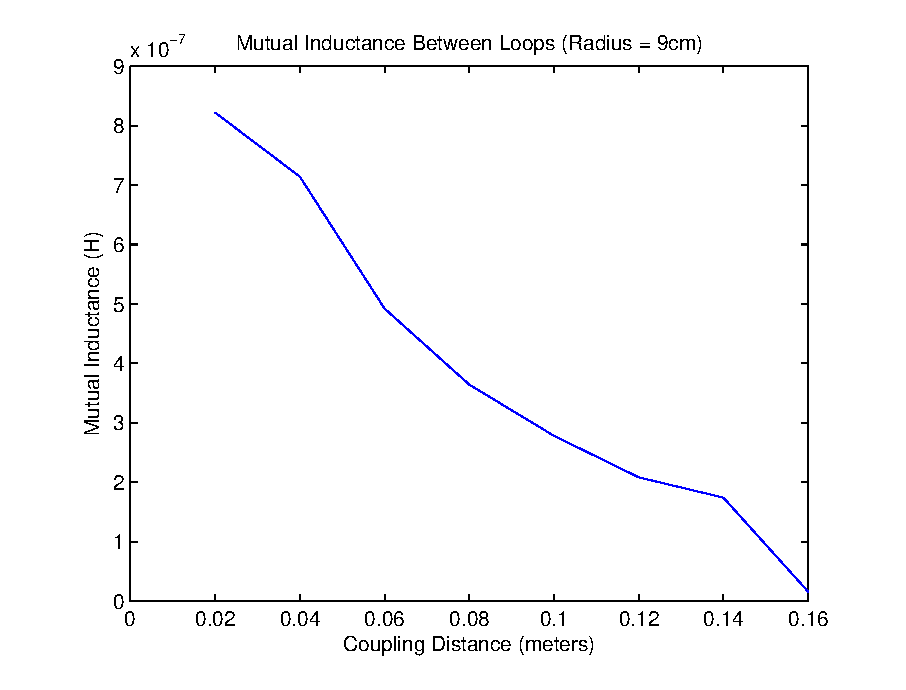
\includegraphics[scale=0.66]{./Matlab/9cm.eps}
	\end{figure}
	\begin{figure}[H]
	\centering
		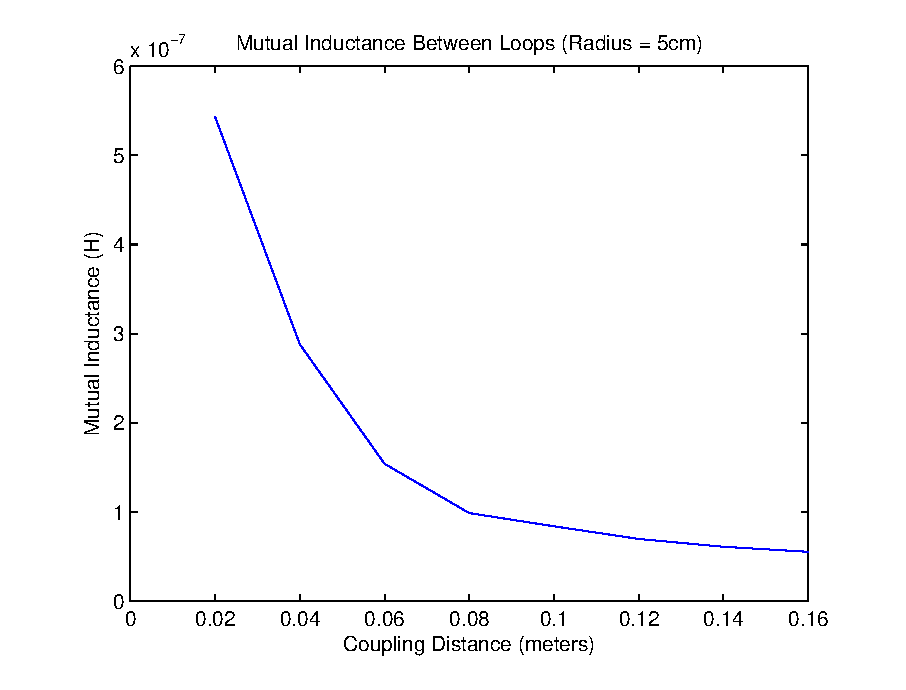
\includegraphics[scale=0.66]{./Matlab/5cm.eps}
	
	\end{figure}
\end{multicols}

\begin{enumerate}
	\item The general decreasing trend is reflected with my measured mutual inductance values, but the data values themselves begin at a higher value and do not decrease as low as the values reflected with the plot. This may be measurement error due to our loops not being perfectly axially-aligned (this was eye-balled). Furthermore, the equations used to generate the provided plots are for filamentary loops; the loops we used in the lab had a non-negligible cross-sectional width and thickness.

	\item
\end{enumerate}


\section{Strong and Weak Coupling}

\subsection{Measured Data}
\begin{table}[H]
\centering
\begin{tabular}{|c|c|c|}
\hline
Loop & Experiment & Theory \\ \hline
9cm & 2cm & \\ \hline
5cm & 1.5cm & \\ \hline
\end{tabular}
\end{table}

\subsection{Analysis}

\begin{enumerate}
	\item Since $\omega M = R + R_L$, $M_{9cm} = 1.01\times10^{-6}$
\end{enumerate}

\subsection{Questions}

\begin{enumerate}
	\item Since $\omega M = R + R_L$, an increase in the resistance of the shielded-loop resonators results in an increase in the mutual inductance; this leads to an increase in the critical coupling distance.
	\item Since $\eta = \dfrac{R_L^2}{(R+R_L)^2}$ under strong coupling, an increase in the resistance of the shielded-loop resonators results in a decrease in power transfer efficiency.
	\item 
	\item
\end{enumerate}


\section{Measuring the Rectifier}

\subsection{Measured Data}

\begin{enumerate}
	\item Rectifier input return loss at $\omega = \omega_0$: -0.47 dB
	\item Rectifier input impedance at $\omega = \omega_0$: 10.07 - j122.6 $\Omega$
\end{enumerate}

\subsection{Questions}

\begin{enumerate}
	\item
\end{enumerate}

\section{Summary}
Pls no.
\end{document}